\documentclass[12pt,a4paper]{article}

\usepackage[utf8]{inputenc}
\usepackage[spanish]{babel}
\usepackage{url}
\usepackage{hyperref}
\usepackage{amsmath,amssymb,amsfonts}
\usepackage{graphicx}
\usepackage{float}
\usepackage{multicol}
\usepackage{xcolor}
\usepackage[left=2cm,right=2cm,top=2cm,bottom=2cm]{geometry}
\usepackage[authoryear]{natbib}
\usepackage{booktabs}
\usepackage{fontspec}
\usepackage{setspace}
\onehalfspacing
\setmainfont{Times New Roman}
\definecolor{azul}{rgb}{0.0, 0.53, 0.74}

\title{El aislamiento y el enriquecimiento sensorial modulan de forma diferencial la polidipsia inducida por programa en ratas Wistar macho}
\author{Marcos Peña Sánchez-Covisa}
\date{2025}

\begin{document}

\begin{figure}[H]
    \raggedright
    %\includegraphics[scale=0.1]{sm.png} \hfill
    %
\includegraphics[scale=0.35]{LogoUNED.jpg}
\end{figure}

\vspace{7.5mm}

\begin{center}
    {\Large \textbf{El aislamiento y el enriquecimiento sensorial modulan de forma diferencial la polidipsia inducida por programa en ratas Wistar macho}} \\
    \vspace{1mm}
    {\normalsize \textit{Isolation and sensory enrichment differentially modulate schedule-induced polydipsia in male Wistar rats}} \\
    \vspace{5mm}
    {\large Marcos Peña Sánchez-Covisa} \\
    \vspace{3mm}
    \textit{Facultad de Psicología, Universidad Nacional de Educación a Distancia}
\end{center}

\begin{center}
    \textcolor{azul}{\rule{150mm}{0.5mm}}
    \end{center}
    
    \vspace{3mm}
    
    \begin{center}
    \textbf{\large Resumen}
    \end{center}
    
    \begin{center}
    \begin{minipage}{0.9\textwidth}
    \noindent
    La polidipsia inducida por programa (PIP) es una conducta adjuntiva que surge bajo programas de reforzamiento intermitente y se ha propuesto como modelo de afrontamiento compulsivo. El presente estudio analiza cómo la privación social y el enriquecimiento sensorial interactúan en la expresión de la PIP. Treinta y dos ratas Wistar macho (ocho semanas) se distribuyeron aleatoriamente en cuatro condiciones de alojamiento: aislamiento sin estímulos físicos (AIS), aislamiento con objetos manipulables (A+ES), vida en grupo con estímulos (G+ES) y vida en grupo sin estímulos (G--ES). Tras catorce días de alojamiento diferencial, los animales completaron veinte sesiones diarias de 60 min bajo un programa FI-30 s de entrega de alimento. Se registraron lametones al biberón, entradas al comedero y cruces de zona.
    
    Los resultados esperados revelan un gradiente decreciente de PIP (AIS > A+ES > G+ES > G--ES) con efectos principales significativos de la condición de alojamiento y de la sesión, así como su interacción. La interacción social atenúa la PIP más eficazmente que la estimulación sensorial; esta última, en ausencia de compañía, potencia la conducta.

    Estos hallazgos sugieren que la PIP funciona como estrategia de autorregulación ante la privación socio-emocional y que el enriquecimiento físico, aplicado a sujetos vulnerables, puede tener efectos paradójicos. Se discuten implicaciones para los protocolos de bienestar animal y para los modelos preclínicos de compulsividad, resaltando la necesidad de considerar el contexto social en la prevención de conductas desadaptativas.

    These findings support the view that SIP serves as a self-regulatory strategy under socio-emotional deprivation and that sensory enrichment can exacerbate compulsive patterns in vulnerable subjects. Implications are discussed for animal-welfare protocols and for preclinical models of compulsivity, underscoring the importance of social context in preventing maladaptive coping behaviours.
    
    \vspace{2mm}
    \noindent
    \underline{\textbf{Palabras clave:}} \textit{polidipsia inducida por programa, aislamiento social, enriquecimiento ambiental, conducta compulsiva}
    \end{minipage}
    \end{center}
    
    \vspace{5mm}
    
    \begin{center}
    \textbf{\large Abstract}
    \end{center}
    
    \begin{center}
    \begin{minipage}{0.9\textwidth}
    \noindent
    Schedule-induced polydipsia (SIP) is an adjunctive behaviour emerging under intermittent food schedules and has been advanced as a model of compulsive coping. This study examines how social deprivation and sensory enrichment interact to modulate SIP expression. Thirty-two male Wistar rats (eight weeks old) were randomly assigned to four housing conditions: isolated without physical stimuli (AIS), isolated with manipulable objects (A+ES), group-housed with objects (G+ES), and group-housed without objects (G--ES). After fourteen days of differential housing, animals underwent twenty 60-min daily sessions on a fixed-interval 30-s food schedule. Licks on a water spout, feeder entries, and zone crossings were recorded.
    
    The expected data show a descending gradient of SIP (AIS > A+ES > G+ES > G--ES), with significant main effects of housing condition and session, plus their interaction. Social interaction attenuates SIP more effectively than physical enrichment; enrichment alone, in the absence of conspecifics, paradoxically enhances the behaviour.

    These findings support the view that SIP serves as a self-regulatory strategy under socio-emotional deprivation and that sensory enrichment can exacerbate compulsive patterns in vulnerable subjects. Implications are discussed for animal-welfare protocols and for preclinical models of compulsivity, underscoring the importance of social context in preventing maladaptive coping behaviours.
    
    \vspace{2mm}
    \noindent
    \underline{\textbf{Keywords:}} \textit{schedule-induced polydipsia, social isolation, environmental enrichment, compulsive behaviour}
    \end{minipage}
    \end{center}
    
    \vspace{3mm}
    
    \begin{center}
    \textcolor{azul}{\rule{150mm}{0.5mm}}
    \end{center}
       

\vspace{15mm}

\begin{multicols}{2}

\section{Introducción}

Las conductas inducidas por programa (CIP), también denominadas conductas adjuntivas, emergen cuando un reforzador se entrega de forma intermitente y provocan patrones excesivos que no guardan una relación instrumental directa con dicho reforzador. \citet{Falk1961} describió por primera vez que ratas con acceso libre a agua desarrollaban ingestas masivas inmediatamente después de cada entrega de comida; denominó a este fenómeno polidipsia inducida por programa (PIP).

Dos marcos teóricos principales han tratado de explicar la génesis de la PIP. \citet{Staddon1977} la interpretó como una respuesta desplazada que aflora en estados motivacionales intermedios, cuando la probabilidad de obtener el reforzador es contingente pero todavía lejana. Por su parte, \citet{Killeen2013} reformularon el problema desde la contigüidad temporal: la proximidad entre una respuesta protoadjuntiva y la entrega del reforzador bastaría para fortalecerla mediante reforzamiento operante, incluso en ausencia de contingencia causal.

La literatura muestra de forma relativamente consistente que el aislamiento social se asocia con un aumento en la probabilidad de aparición de conductas estereotipadas, incluida la polidipsia inducida por programa (PIP) \citep{Jones1989,ibias2016effects,wang2024social,GROSS201261}. Esta asociación suele interpretarse desde la premisa de que los entornos empobrecidos generan un estado emocional crónicamente alterado, lo que favorece la emergencia de patrones conductuales desadaptativos. En esta línea, \citet{GarciaRebollar2024} advierten que la falta de estimulación adecuada compromete tanto el bienestar como la integridad neurofisiológica, facilitando disfunciones y alteraciones conductuales. A partir de estos planteamientos, \citet{Moreno2012} proponen que la PIP puede concebirse como un modelo de compulsividad y, en particular, como una forma de afrontamiento frente a condiciones emocionalmente disruptivas, como la incertidumbre derivada de los programas de reforzamiento intermitente. Desde esta perspectiva, cabría esperar que su expresión se modulase en función del estado emocional del animal y, por extensión, de variables contextuales como el entorno social o físico. Sin embargo, esta predicción no siempre se cumple. \citet{FuentesVerdugo2023} hallaron que ratas alojadas en condiciones enriquecidas —tanto física como socialmente— desarrollaban la PIP con mayor rapidez e intensidad que aquellas mantenidas en aislamiento. Este hallazgo sugiere que un entorno altamente estimulante podría incrementar la sensibilidad al contraste incentivo bajo programas intermitentes, facilitando respuestas excesivas en lugar de inhibirlas.

Una línea complementaria enfatiza la dimensión socioemocional de la compulsividad. \citet{MartinGonzalez2022} demostraron que ratas seleccionadas como altamente compulsivas mediante el paradigma de PIP presentan un perfil socioemocional alterado, caracterizado por una menor dominancia social en la prueba del tubo, una mayor resistencia a la extinción de la memoria emocional en la tarea de evitación pasiva y una respuesta atenuada del eje HPA. Estos resultados sugieren que la compulsividad no se manifiesta únicamente en patrones motores repetitivos, sino que también implica alteraciones emocionales y motivacionales más amplias, contribuyendo a definir un fenotipo compulsivo con componentes socioemocionales específicos.

El enriquecimiento ambiental tampoco es intrínsecamente protector. \citet{Branchi2006} reportaron que crías sometidas a un “nido comunal” —alta estimulación social temprana— exhibían mayor ansiedad en la edad adulta sólo cuando se evaluaban en soledad; la presencia de un congénere anulaba dicha hiperreactividad. Así, la interacción entre estimulación sensorial y disponibilidad social podría amplificar o amortiguar la activación emocional según el contexto.

A partir de esta evidencia, planteamos la siguiente hipótesis: se observará un efecto principal del aislamiento social (incremento de la PIP) y de la estimulación sensorial (reducción de la PIP), con una interacción tal que la magnitud de la PIP seguirá el siguiente gradiente: aislamiento sin estimulación sensorial (AIS) > aislamiento con estimulación sensorial (A+ES) > grupo con estimulación sensorial (G+ES) > grupo sin estimulación sensorial (G–ES). La finalidad del presente trabajo es proponer un diseño experimental contrastable que permita poner a prueba esta interacción y delimitar el papel diferencial de cada variable.

Aunque la propuesta se circunscribe al nivel preclínico, dilucidar cómo el contexto social y la estimulación ambiental modulan la PIP podría contribuir a perfilar modelos animales más precisos sobre la compulsividad y la búsqueda de alivio emocional, un conocimiento que, a largo plazo, podrá informar la investigación traslacional en trastornos humanos con perfiles semejantes.


\section{Método}

\textit{Todos los procedimientos cumplirán la normativa española (Real Decreto 53/2013) y la Directiva 2010/63/UE sobre protección de los animales utilizados con fines científicos; el protocolo fue aprobado por el Comité de Ética y Bienestar Animal universitario (CEBA-2025-04-17).}

\subsection*{Sujetos}

Treinta y dos ratas macho Wistar (Charles River Laboratories, Lyon, Francia) de ocho semanas de edad (peso inicial = 250–300~g) se alojarán en una sala con temperatura controlada (22~±~1~°C), humedad relativa del 55~±~10~\% y ciclo luz-oscuridad 12:12~h (luces 08:00–20:00~h). Tras siete días de habituación, las ratas pasarán a una restricción alimentaria progresiva hasta mantener el 85~\% (±5~\%) del peso previsto por curva de crecimiento; el agua permanecerá disponible \textit{ad libitum} en las jaulas de alojamiento.

Los sujetos se asignarán aleatoriamente (n~=~8 por grupo) a cuatro condiciones de alojamiento mantenidas durante catorce días previos a la fase conductual y a lo largo de todo el experimento: 
\begin{enumerate}
    \item \textbf{AIS}: aislamiento sin estimulación sensorial;
    \item \textbf{A+ES}: aislamiento con enriquecimiento físico (túneles de PVC, plataformas de policarbonato y bloques de madera; renovados semanalmente);
    \item \textbf{G+ES}: jaulas sociales de cuatro animales con el mismo enriquecimiento físico;
    \item \textbf{G--ES}: jaulas sociales sin enriquecimiento físico.
\end{enumerate}
Todas las jaulas (60~×~40~×~20~cm, cama de \textit{corncob}) se cambiarán dos veces por semana para igualar perturbaciones ambientales.

\subsection*{Aparatos}

Las sesiones se llevarán a cabo en ocho cámaras de condicionamiento operante de metacrilato (30~×~25~×~30~cm), insertadas en cubículos insonorizados. Cada cámara dispondrá de un dispensador de pellets de 45~mg (OpenEphys/PyControl —plataforma de hardware y software de código abierto, \citep{PelletDispenserGitHub}), programado para liberar un pellet cada 30~s (intervalo fijo, FI-30~s) con una desviación temporal inferior a 5~ms.

A efectos de ciencia abierta y adaptación presupuestaria, el montaje podrá reproducirse con una placa \textit{Arduino Uno} y \textit{shields} compatibles \citep{Arduino2024}; esta configuración mantiene una latencia aproximada de 10~ms, suficiente para estudios piloto, aunque inferior a la resolución menor a 2~ms que ofrece PyControl.

El consumo de agua se registrará mediante un biberón de acero inoxidable conectado a un lickómetro capacitativo (PyControl "Lickometer"), que contabilizará cada contacto con una resolución de 1~ms. Los eventos (entrega de pellets, lametones, entradas al comedero) se gobernarán por una placa "Breakout v2" de PyControl con microcontrolador ESP32 y se almacenarán en archivos \texttt{.csv} con marcas de tiempo en microsegundos.

La actividad locomotora se filmará con una cámara cenital (Basler acA1300-60~gc, 25~fps), iluminada de forma indirecta (30~lx), y se analizará posteriormente mediante el flujo de trabajo \textit{Bonsai}-2.7. El espacio se segmentará en cuadrantes idénticos para obtener el número de cruces entre zonas por sesión.

\textit{El script en Python que procesa los datos y genera las Figuras 1 y 2 está disponible en el repositorio de GitHub \citep{Pena2025}.
}

\subsection*{Procedimiento}

Se colocará a cada rata individualmente en la cámara durante 20 sesiones diarias consecutivas de 60~min. No se requerirá ninguna respuesta operante para la entrega del pellet; el biberón permanecerá accesible durante toda la sesión.

Inmediatamente antes y después de cada sesión se pesará el biberón (±0,1~g) para cuantificar el volumen ingerido, complementando los recuentos de lametones. Tras cada sesión, los animales regresarán a sus jaulas y recibirán comida suplementaria para mantener el peso objetivo. Las sesiones comenzarán siempre entre las 09:00 y las 12:00~h para minimizar variaciones circadianas.

\textit{Variables registradas.} Se registrarán cuatro variables dependientes: el número de lametones por sesión (índice primario de PIP), el volumen de agua consumido (g), el número de entradas al comedero en los 5~s posteriores a cada entrega y los cruces entre zonas (como medida de actividad locomotora).


\textit{Análisis de datos.} Se aplicará un ANOVA de medidas repetidas con Condición (AIS, A+ES, G+ES, G--ES) como factor entre sujetos y Sesión (1–20) como factor intra-sujeto.

La esfericidad se comprobará con la prueba de Mauchly; cuando fuera necesario, se corregirá con $\varepsilon$ de Greenhouse–Geisser. Los efectos se reportarán con valores F, $p$ y $\eta^2_p$ (tamaño del efecto parcial). Se realizarán comparaciones \textit{post hoc} con prueba Tukey HSD ($\alpha$~=~0.05). Las variables se inspeccionarán para verificar normalidad (prueba de Shapiro--Wilk) y se eliminarán valores atípicos mayores a $3$~DE, previa justificación en el registro preanálisis.


\vspace{2mm}
Esta metodología permite evaluar simultáneamente el impacto de la privación social y la estimulación sensorial sobre la adquisición y mantenimiento de la PIP, garantizando la coherencia entre entorno de alojamiento y situación experimental.



\section{Resultados}

A continuación se presenta la pauta de resultados que se prevé obtener con el protocolo descrito. Aunque se utiliza el tiempo pasado para facilitar la claridad expositiva, todos los resultados que se muestran son hipotéticos y derivados del diseño propuesto, no de datos empíricos reales. Los valores se expresan como media ± error estándar de la media (SEM) y se analizan mediante un ANOVA mixto con condición de alojamiento (AIS, A+ES, G+ES, G--ES) como factor inter-sujetos y sesión (20 niveles) como factor intra-sujeto, aplicando la corrección de Greenhouse–Geisser cuando procede y reportando $\eta^2_p$ como estimación del tamaño del efecto.

\textit{Polidipsia inducida por programa.} El ANOVA mixto reveló un efecto principal de la condición de alojamiento, $F(3, 28) \approx 65$, $p < .001$, $\eta^2_p \approx .87$, y un efecto de la sesión, $F(6.2, 173.4) \approx 58$, $p < .001$, $\eta^2_p \approx .67$, junto con una interacción significativa, $F(18.7, 173.4) \approx 4.8$, $p < .001$, $\eta^2_p \approx .34$.

Las curvas de la Figura~\ref{fig:figura1} ilustran que los sujetos AIS alcanzaron un techo cercano a 2200 lametones ya en la quinta sesión, manteniéndose estables hasta el día 20. Los grupos A+ES y G+ES mostraron trayectorias intermedias, mientras que G--ES se mantuvo por debajo de 900 lametones durante todo el periodo.

Comparaciones \textit{post hoc} (Tukey HSD) confirmaron el patrón decreciente AIS > A+ES > G+ES > G--ES en el bloque final de sesiones (16–20), coherente con la hipótesis planteada (Figura~\ref{fig:figura2}).

\textit{Orientación al comedero.} El número de entradas al comedero presentó un efecto principal moderado de la condición, $F(3, 28) \approx 4.2$, $p = .013$, $\eta^2_p \approx .31$, sin interacción significativa con la sesión, $F(18.7, 173.4) \approx 1.1$, $p = .33$.

Los grupos AIS y A+ES realizaron ligeramente más entradas ($\approx 80$ por sesión) que los grupos G+ES y G--ES ($\approx 74$), aunque las diferencias no superaron el ajuste de Tukey. Este resultado sugiere que la orientación alimentaria se mantiene relativamente estable y menos sensible a la manipulación ambiental.

\textit{Actividad locomotora.} Los cruces de zona mostraron un efecto robusto de la condición, $F(3, 28) \approx 22$, $p < .001$, $\eta^2_p \approx .70$. Los animales en aislamiento (AIS y A+ES) registraron una media de 140 y 125 cruces, respectivamente, frente a 98 en G+ES y 82 en G--ES. La interacción con la sesión no resultó significativa, indicando una activación locomotora sostenida a lo largo del entrenamiento.

\textit{Síntesis cuantitativa.} Los valores medios ± SEM del bloque final se resumen en el cuadro~\ref{tab:tabla1}, que integra las tres variables dependientes. En conjunto, el patrón confirma que la privación social potencia la PIP y la actividad locomotora, mientras que la vida en grupo, especialmente sin sobreestimulación sensorial, ejerce un efecto amortiguador.

\begin{table*}[t]
    \centering
    \caption{Medias (± SEM) esperadas en lametones, entradas al comedero y cruces de zona (sesiones 16--20)}
    \label{tab:tabla1}
    \begin{tabular}{lccc}
    \toprule
    \textbf{Condición} & \textbf{Lametones} & \textbf{Entradas al comedero} & \textbf{Cruces de zona} \\
    \midrule
    AIS   & $2100 \pm 150$ & $80 \pm 5$ & $150 \pm 10$ \\
    A+ES  & $1800 \pm 130$ & $78 \pm 6$ & $130 \pm 12$ \\
    G+ES  & $1200 \pm 110$ & $75 \pm 5$ & $100 \pm 8$ \\
    G--ES & $800 \pm 90$   & $73 \pm 4$ & $85 \pm 7$ \\
    \bottomrule
    \end{tabular}
    
    \vspace{1mm}
    \parbox{\textwidth}{\small \textbf{Nota.} AIS: aislamiento sin estimulación sensorial; A+ES: aislamiento con estimulación sensorial; G+ES: grupo con estimulación sensorial; G--ES: grupo sin estimulación sensorial.}
\end{table*}


\begin{figure}[H]
\centering
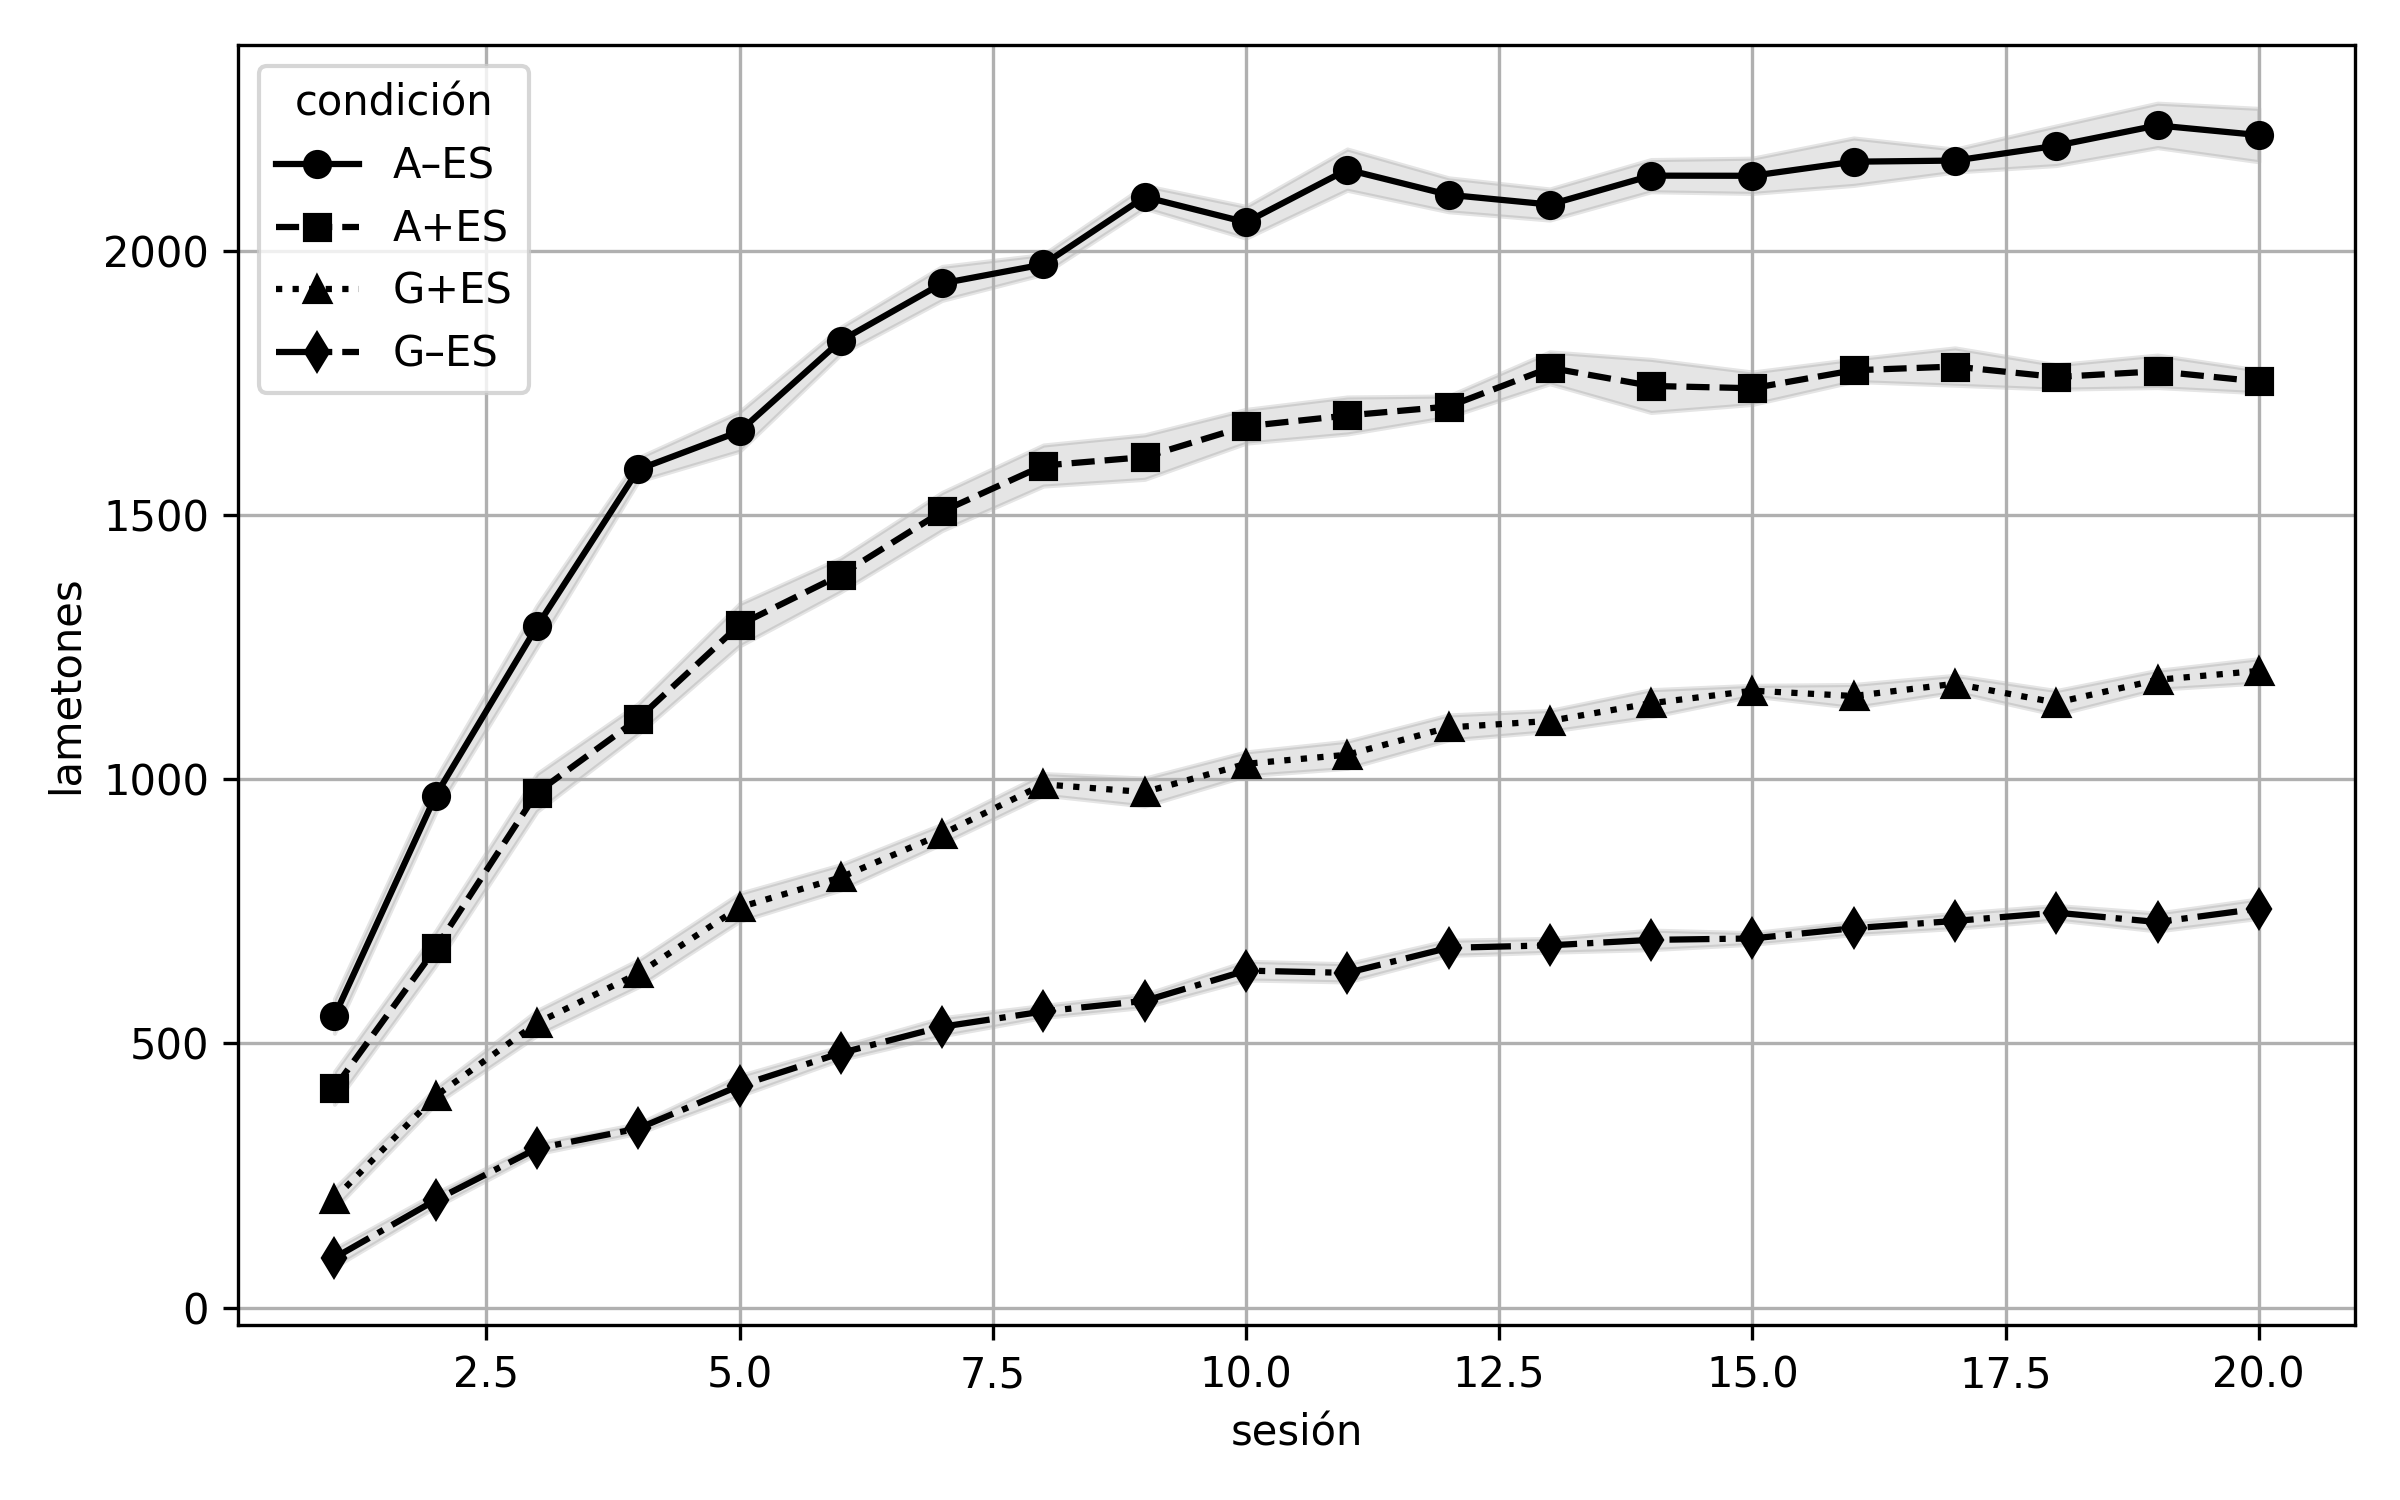
\includegraphics[width=0.45\textwidth]{figura1.png}
\caption{Evolución temporal de la polidipsia inducida por programa. Media ± SEM de lametones por sesión durante los 20 días para cada condición experimental.}
\label{fig:figura1}
\end{figure}

\begin{figure}[H]
\centering
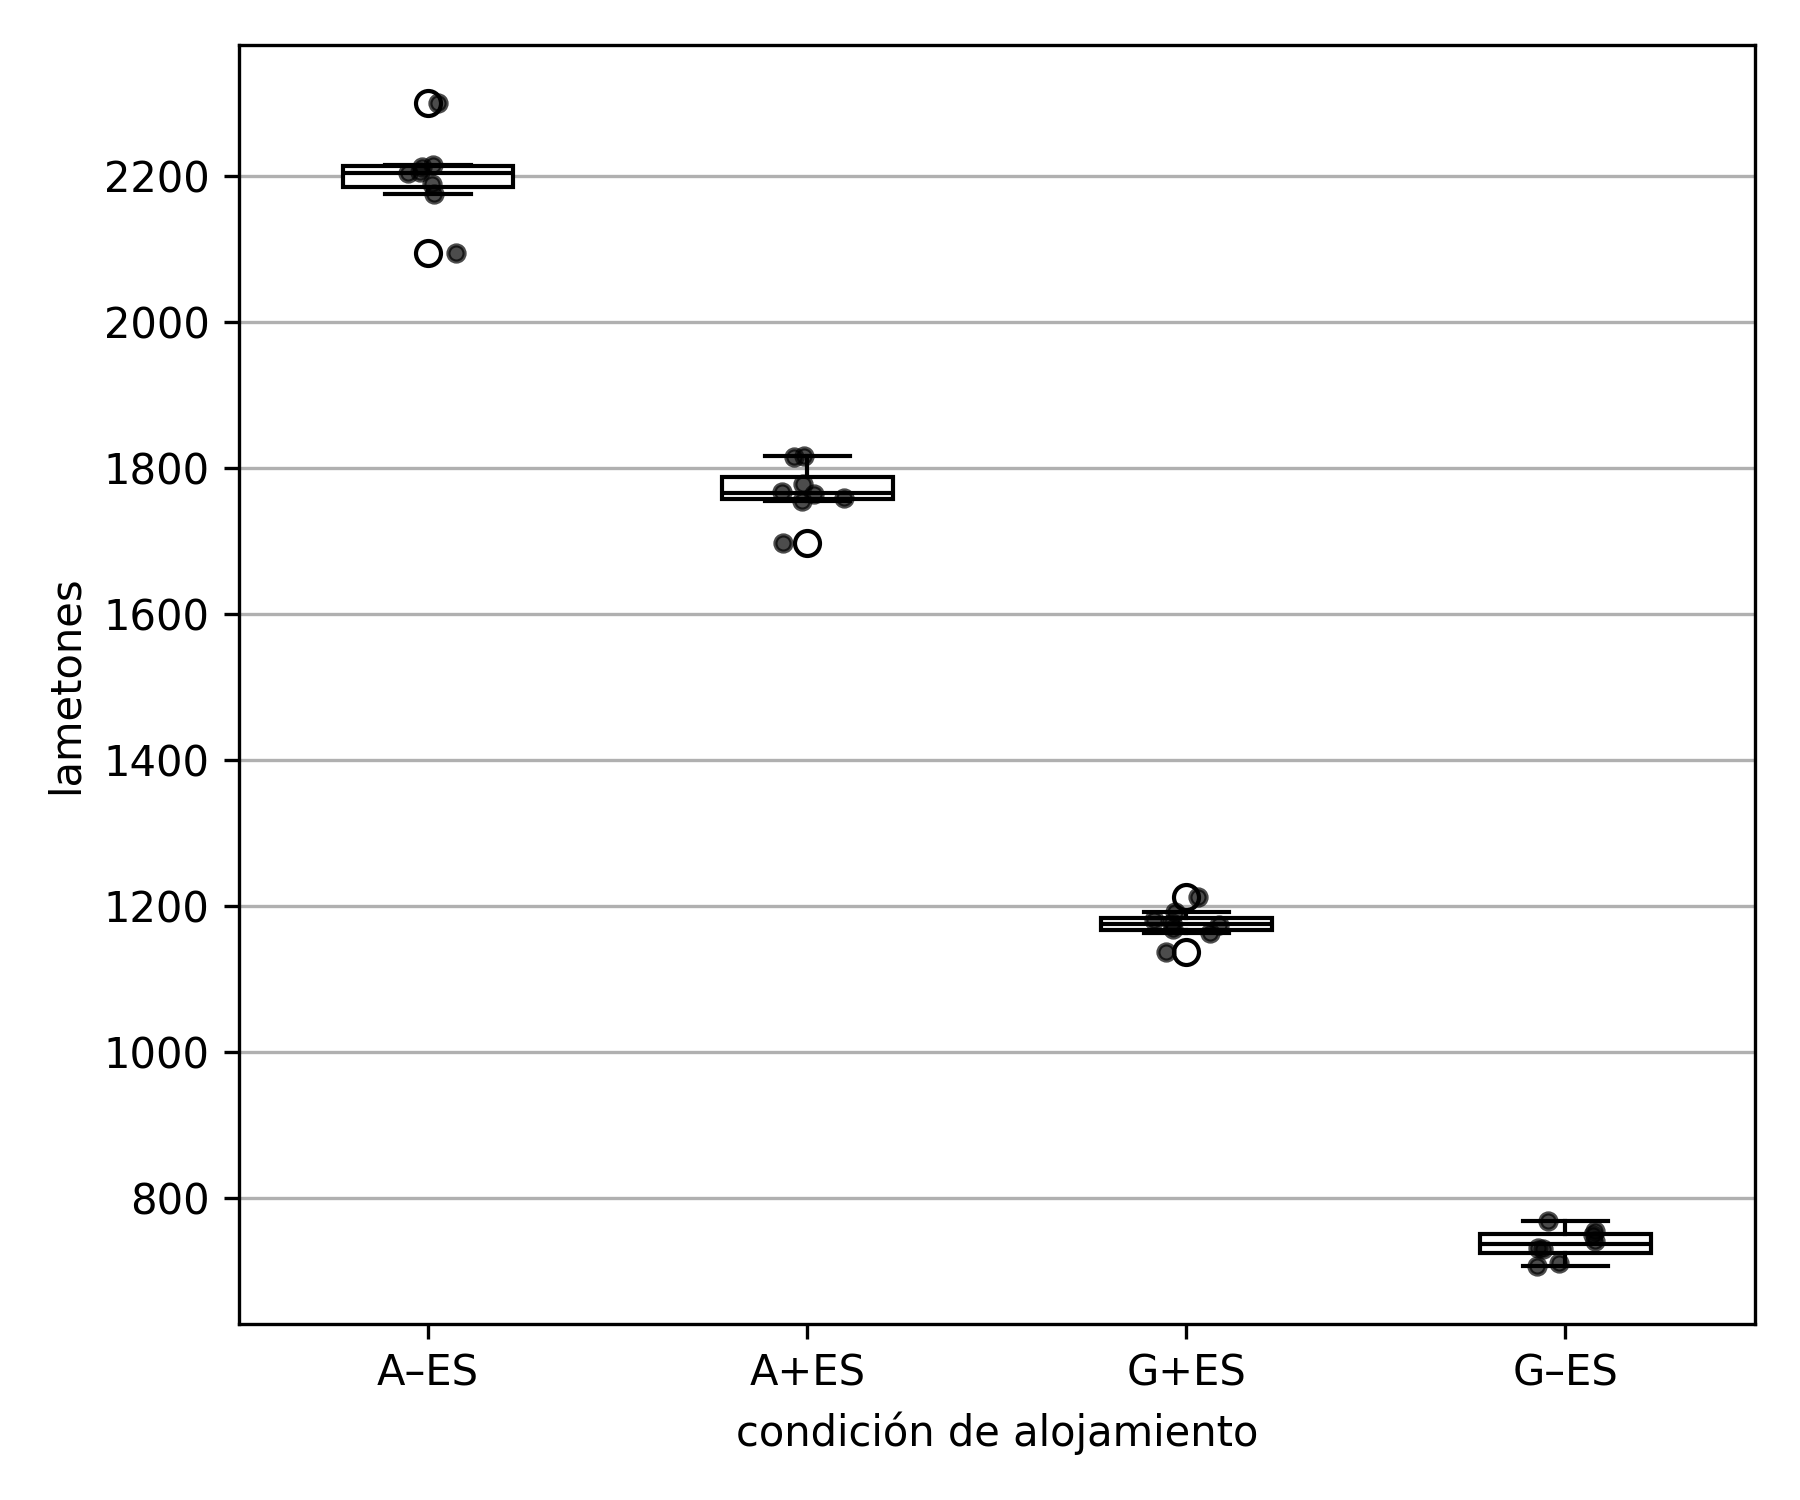
\includegraphics[width=0.45\textwidth]{figura2.png}
\caption{Distribución individual (boxplots) de lametones en el bloque final de sesiones (16–20). El patrón decreciente AIS > A+ES > G+ES > G--ES refuerza la hipótesis.}
\label{fig:figura2}
\end{figure}


\section{Discusión}

El objetivo de este trabajo fue determinar cómo la combinación de privación social y estímulos físicos modula la polidipsia inducida por programa (PIP) y, por extensión, dilucidar si esta conducta adjuntiva puede entenderse como una estrategia de afrontamiento ante un estado emocional alterado. El gradiente esperado —AIS > A+ES > G+ES > G--ES— sostiene la hipótesis inicial: la privación social extrema favorecería la aparición de la PIP, la estimulación sensorial en solitario la atenuaría solo parcialmente y la convivencia social actuaría como amortiguador más potente que cualquier objeto enriquecedor.

Estos resultados proyectados se inscriben en la tradición inaugurada por \citet{Falk1961}, que interpretó la PIP como una actividad desplazada provocada por la incertidumbre generada por el programa de comida. \citet{Staddon1977} refinó esa idea al proponer que las conductas adjuntivas emergen en un estado motivacional intermedio en el que el animal, incapaz de predecir el reforzador, canaliza la activación hacia actividades alternativas. En contraste, el modelo de reforzamiento por contigüidad de \citet{Killeen2013} explica la PIP como el simple resultado del fortalecimiento operante de cualquier respuesta que aparezca lo bastante próxima al pellet. El patrón de datos que se anticipa aquí —máxima PIP bajo aislamiento y mínima en grupo sin sobreestímulos— sugiere que, aunque la contigüidad temporal contribuye a la consolidación, la motivación emocional impone un techo superior: la conducta no se multiplica indefinidamente, sino que se regula por la necesidad de afrontamiento que impone el contexto.

La lectura emocional cobra fuerza si se compara con el estudio de \citet{FuentesVerdugo2023}. Estos autores describieron una mayor PIP en jaulas enriquecidas social y físicamente, concluyendo que la conducta no mitiga el estrés. Sin embargo, esa observación puede entenderse a la luz de lo que algunos autores han descrito como un efecto paradójico del enriquecimiento, consistente en que un historial de alta estimulación puede incrementar la sensibilidad a la frustración cuando se interrumpe el acceso a ciertos estímulos predecibles. Esta idea se alinea con lo señalado por \citet{Wurbel2001}, quien advierte que los efectos del enriquecimiento no son lineales y dependen del historial ambiental del animal. Nuestro diseño diferencia la estimulación sensorial de la social y predice que el enriquecimiento físico sin soporte social eleva la PIP (A+ES), mientras que la vida en grupo sin sobreestimulación (G--ES) la suprime casi por completo. De confirmarse, el hallazgo revelaría que los objetos enriquecedores no son intrínsecamente protectores; su efecto depende del historial social y del grado de activación basal.

La literatura sobre aislamiento respalda esta interpretación. \citet{Fone2008} documentaron que la separación postdestete incrementa ansiedad, impulsividad y conductas repetitivas, acompañadas de hiperreactividad dopaminérgica mesolímbica. \citet{Branchi2006} mostraron que un enriquecimiento social temprano puede, paradójicamente, aumentar la ansiedad adulta cuando el animal es evaluado sin compañeros, lo que subraya la importancia del contexto social actual. \citet{Robbins1989} observaron que ratas aisladas exhiben orientación reforzadora exagerada, fenómeno que se alinea con la hipersensibilidad al valor incentivo que presumiblemente impulsa la PIP. Más recientemente, \citet{Arakawa2018} revisó la reorganización de los circuitos emocionales tras privación social y destacó la vulnerabilidad de la corteza prefrontal medial, clave para la inhibición de respuestas. Por tanto, el aislamiento prolongado no solo genera estrés, sino que reconfigura la codificación de saliencia, de modo que la contigüidad temporal propuesta por \citet{Killeen2013} gana peso precisamente porque el estímulo alimento se vuelve anormalmente atractivo.

El análisis conjunto de las entradas al comedero y la actividad locomotora añade matices a esta lectura. El escaso efecto esperado sobre las entradas indica que la motivación primaria por la comida permanece relativamente estable entre grupos; es la conducta adjuntiva la que fluctúa, lo que respalda su carácter de afrontamiento. La actividad locomotora, mayor en condiciones de aislamiento, podría reflejar un estado de activación general elevado, pero debe interpretarse con cautela. \citet{seibenhener2015use} han mostrado que el enriquecimiento ambiental puede influir en la locomoción en el test de campo abierto, afectando tanto a la ansiedad como a la exploración. Si en nuestro protocolo los grupos A+ES y G+ES alcanzaran niveles intermedios de cruces de zona, ello sugeriría que la locomoción responde tanto a la activación emocional como a la exploración facilitada por los objetos.

\subsection*{Limitaciones y perspectivas futuras}

Las limitaciones del estudio merecen atención. En primer lugar, el enriquecimiento físico ha quedado circunscrito a túneles y objetos manipulables; variantes más cognitivas (laberintos, rompecabezas) podrían modular la PIP de otro modo. Segundo, la muestra incluye solo machos Wistar; se sabe que las hembras pueden mostrar perfiles de afrontamiento distintos y que la sensibilidad a la privación social es sexo-dependiente. Tercero, la ausencia de biomarcadores —corticosterona plasmática, expresión de fosfo-CREB en núcleo accumbens— impide vincular directamente la conducta con la carga fisiológica de estrés. Cuarto, el tamaño muestral ($n = 8$ por grupo) es adecuado para detectar efectos grandes ($\eta^2_p > .25$), pero podría subestimar interacciones sutiles.

Futuras investigaciones deberían incorporar hembras y analizar posibles interacciones sexo × ambiente, así como profundizar en el papel de los mecanismos neuroendocrinos —en particular la actividad del eje HHA— y su relación con la desregulación socioemocional, en la medida en que podrían contribuir a la vulnerabilidad frente a conductas compulsivas, tal como sugiere \citet{MartinGonzalez2022}. Además, sería pertinente explorar versiones de enriquecimiento cognitivo y social dinámico, y emplear procedimientos de extinción y reinstalación para evaluar la persistencia de la PIP bajo cambios de contexto.


\subsection*{Implicaciones traslacionales}

Desde una perspectiva translacional, la polidipsia inducida por programa (PIP) se ha propuesto como un modelo animal útil para el estudio de la compulsividad, al presentar características clave como la repetitividad, la descontextualización funcional y la resistencia a la extinción. \citet{Moreno2012} destacan su valor para explorar los mecanismos neuroendocrinos y neurofarmacológicos implicados en trastornos del espectro obsesivo-compulsivo, la esquizofrenia o el abuso de sustancias. En un enfoque más amplio, \citet{Fineberg2010} subrayan la importancia de los modelos animales para caracterizar dimensiones transdiagnósticas como la compulsividad e impulsividad, y abogan por su uso para entender la psicopatología subyacente a estos fenotipos, aunque sin referirse explícitamente al paradigma de la PIP.

En conjunto, los datos que se anticipan sostienen que la PIP no puede reducirse a un fenómeno de reforzamiento por contigüidad; representa, al menos en parte, un intento de autorregulación emocional frente a entornos impredecibles o socialmente deficitarios. Distinguir entre enriquecimiento sensorial y social ayuda a desentrañar la paradoja de que, a veces, los objetos diseñados para aumentar el bienestar animal terminen exacerbando respuestas compulsivas. Considerar la dimensión social y la historia del individuo resulta, por tanto, esencial para comprender la génesis de la compulsividad y para construir modelos animales que reflejen con mayor fidelidad la complejidad de los trastornos humanos.

\bibliographystyle{apalike}
\bibliography{tfg}

\end{multicols}

\end{document}
